\subsection{Hiện thực quầy và cập nhật theo thời gian thực}
\label{sec:staff-implementation}
\subsubsection{Kiểm soát chuyển trạng thái tại backend}
StaffOrdersController nhận PATCH trạng thái qua JwtAuthGuard/RolesGuard; DTO chỉ nhận PREPARING, READY hoặc COMPLETED. OrdersService.updateStaffStatus khóa Order, đọc lại trạng thái, kiểm yêu cầu đổi chờ và gọi assertTransition. UPDATE kèm điều kiện trạng thái hiện tại, kiểm count trước khi commit. Hai request cùng duyệt một đơn PAID sang PREPARING chỉ có một request hợp lệ; request tiếp theo không được coi PREPARING sang PREPARING là bước mới.

Máy trạng thái là luật chuyển tiếp dùng chung, còn quyền và điều kiện cụ thể nằm ở service. Có cạnh PAID sang CANCELLED không có nghĩa API quầy được hủy tùy ý: luồng đổi món/hủy/hết hạn có kiểm tra riêng. Các phần xử lý tài chính và kho được tham chiếu ở những mục tương ứng, không thực hiện lại khi bấm ``Pha xong'' hoặc ``Đã giao khách''.

\subsubsection{Thông báo sau commit và tải lại dữ liệu}
OrdersGateway dùng namespace /orders-live, phát orders.changed không payload. notifyOrdersChanged được gọi sau transaction thành công; rollback hoặc replay không làm một kết quả chưa commit xuất hiện như thành công trên màn hình khác.

Hook useOrdersLive đăng ký connect/disconnect/connect\_error và orders.changed. Khi kết nối hoặc nhận sự kiện, client tải lại API. Có polling HTTP 15 giây khi tab hiển thị và nút tải lại để hỗ trợ khi mất kênh tức thời. Mỗi refresh hủy request trước bằng AbortController; cleanup gỡ listener, ngắt socket và dọn interval khi component rời màn hình. Thanh trạng thái kết nối chỉ biểu diễn kênh cập nhật, không chứng minh một đơn đã trả tiền hoặc đã pha.

\begin{figure}[htbp]\centering
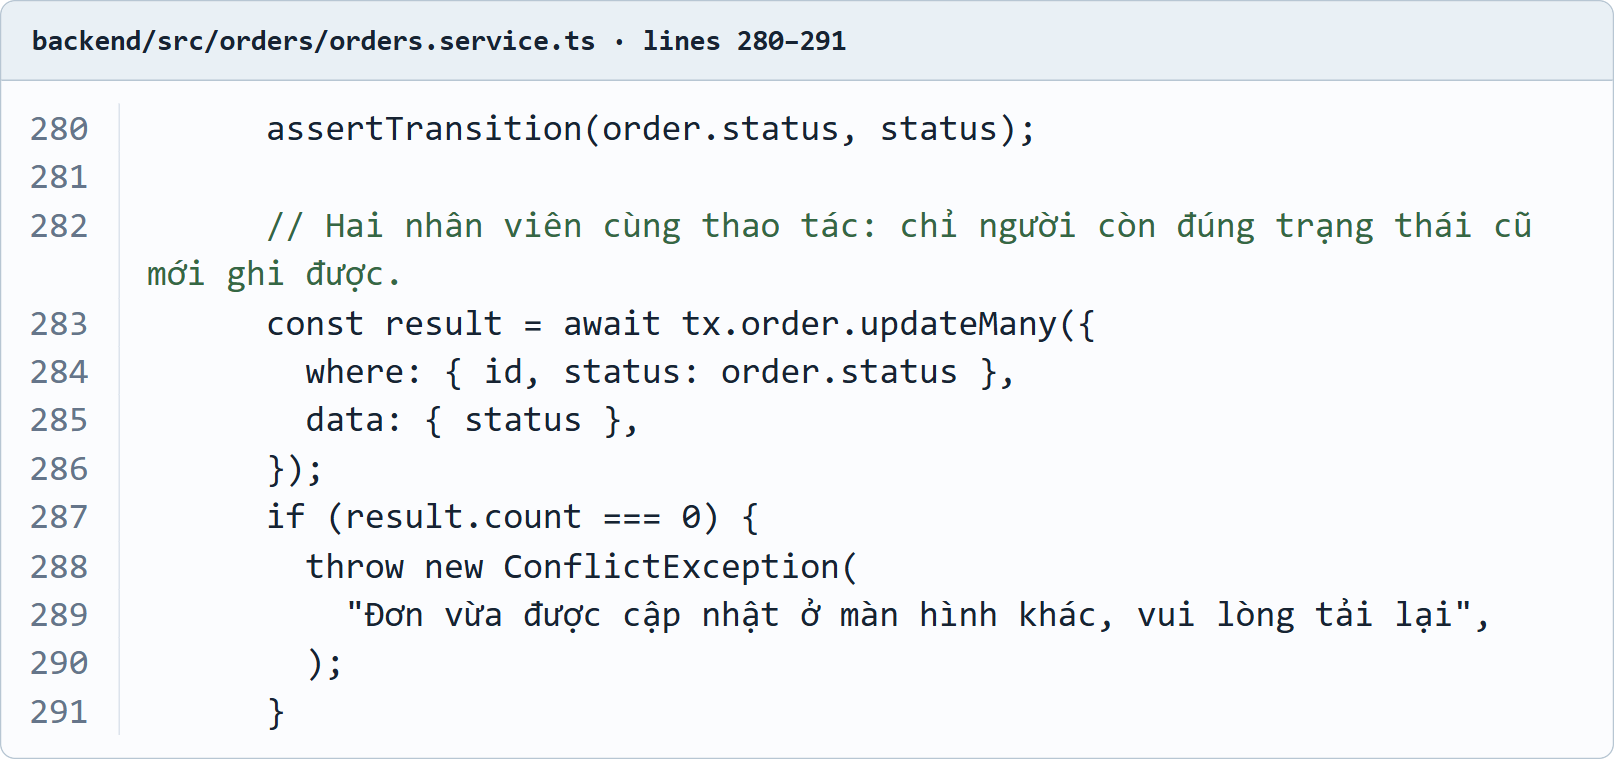
\includegraphics[width=.94\linewidth,height=.25\textheight,keepaspectratio]{assets/staff/code-transition.png}
\caption{Cập nhật có điều kiện sau khi kiểm luật chuyển tiếp và khóa Order}
\vspace{3mm}
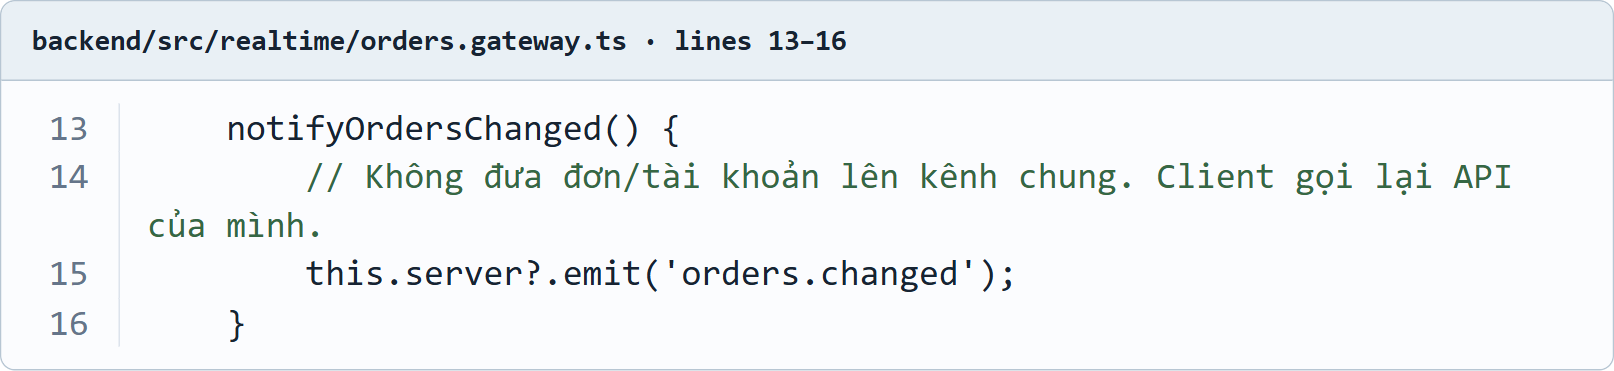
\includegraphics[width=.94\linewidth,height=.16\textheight,keepaspectratio]{assets/staff/code-event.png}
\caption{Gateway chỉ phát tín hiệu thay đổi, không đưa dữ liệu đơn lên kênh chung}
\vspace{3mm}
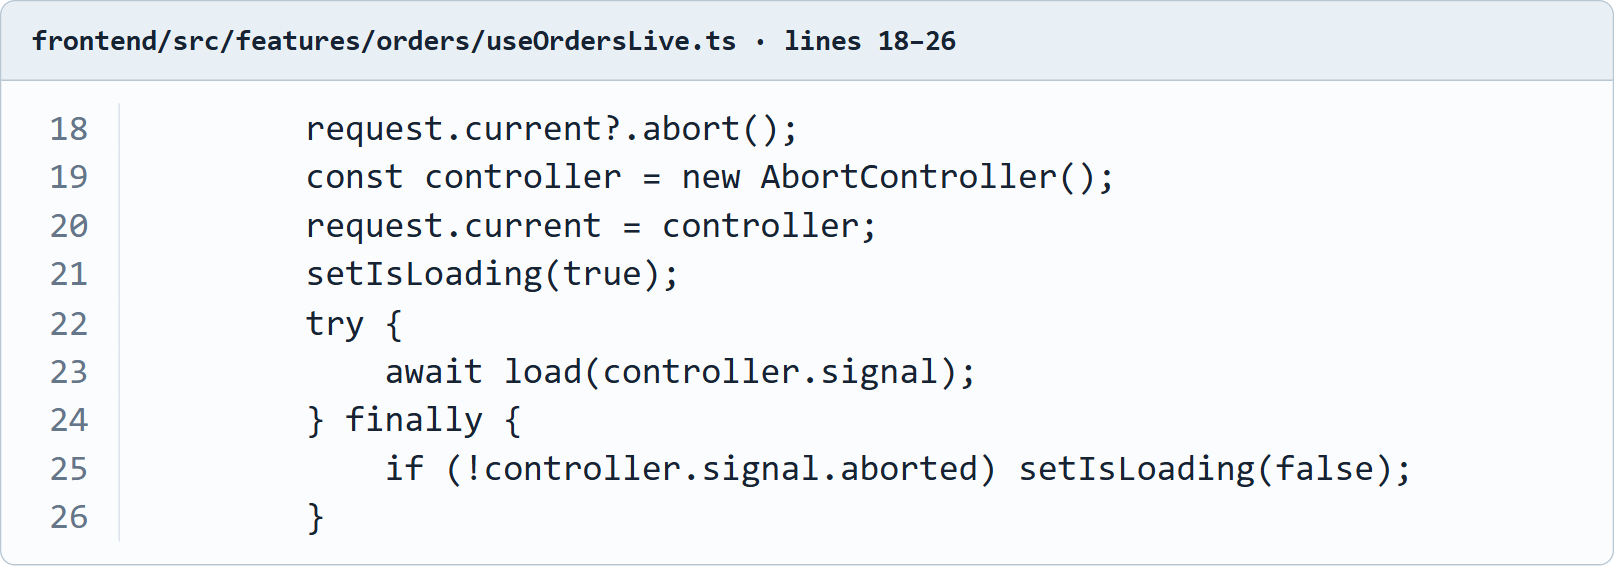
\includegraphics[width=.94\linewidth,height=.25\textheight,keepaspectratio]{assets/staff/code-refresh.png}
\caption{Client chỉ giữ request tải mới và hủy request cũ khi refresh}
\end{figure}
